
\documentclass[twocolumn]{article}
\usepackage{mathpazo}
\usepackage{microtype}
\usepackage{times}
\usepackage{titlesec} % 1
%\usepackage{sectsty} % "제 1 절" ...

 %%%%%%%%%%%%%%%%%%%%%%%%%%%%%%%%%%%%%%%%%%%%%%%%%%%%%%%%%%%%%%%%%%%%%%%%%%%%%
 %                              My Commands
\newcommand{\bi}{\begin{itemize}}
\newcommand{\ei}{\end{itemize}}
\newcommand{\be}{\begin{enumerate}}
\newcommand{\ee}{\end{enumerate}}
\newcommand{\ii}{\item}
\newtheorem{Def}{Definition}
\newtheorem{Lem}{Lemma}
\usepackage{algorithm}
\usepackage{algorithmicx}
\usepackage{algpseudocode}

\usepackage{graphicx}
\graphicspath{%
        {converted_graphics/}
        {./images/}
}

\usepackage{color}
\usepackage{xcolor}
\usepackage{listings}
\usepackage{caption}
\DeclareCaptionFont{white}{\color{white}}
\DeclareCaptionFormat{listing}{\colorbox{gray}{\parbox{\textwidth}{#1#2#3}}}
\captionsetup[lstlisting]{format=listing,labelfont=white,textfont=white}
\usepackage{verbatimbox}

\usepackage[hangul,nonfrench,finemath]{kotex}
    
\setlength\textwidth{7in} 
\setlength\textheight{9.5in} 
\setlength\oddsidemargin{-0.25in} 
\setlength\topmargin{-0.25in} 
\setlength\headheight{0in} 
\setlength\headsep{0in} 
%\setlength\columnsep{5pt}
\sloppy 
 
\begin{document}

\title{
\vspace{-0.5in}\rule{\textwidth}{2pt}
\begin{tabular}{ll}\begin{minipage}{4.75in}\vspace{6px}
\noindent\large {\it KIWI Project}@Data Management Research Section\\
\vspace{-12px}\\
\noindent\LARGE ETRI\qquad  \large Technical Report 15ZS1410-TR-62
\end{minipage}&\begin{minipage}{2in}\vspace{6px}\small
218 Gajeong-ro, Yuseong-gu\\
Daejeon, 305-700, South Korea\\
http:/$\!$/www.etri.re.kr/\\
http:/$\!$/sungsoo.github.com/\quad 
\end{minipage}\end{tabular}
\rule{\textwidth}{2pt}\vspace{0.25in}
\LARGE \bf 아파치 하이브에서 질의 처리 구현 상세 \\
\large Implementation Details of Query Processing in Apache Hive
}

\date{}

\author{
{\bf Sung-Soo Kim}\\
\it{sungsoo@etri.re.kr}
}

\maketitle

\begin{abstract}
아파치 하이브(Apache Hive)는 하둡에서 동작하는 데이터 웨어하우스(Data Warehouse) 인프라 구조로서 데이터 요약, 질의 및 분석 기능을 제공한다. 초기에는 페이스북에서 개발되었지만 넷플릭스등과 같은 회사에서 사용되고 있으며 개발되고 있다. 
아파치 하이브는 아파치 HDFS이나 아파치 HBase와 같은 데이터 저장 시스템에 저장되어 있는 대용량 데이터 집합들을 분석한다. HiveQL 이라고 불리는 SQL같은 언어를 제공하며 맵리듀스의 모든 기능을 지원한다. 쿼리를 빠르게 하기위해 비트맵 인덱스를 포함하여 인덱스 기능을 제공한다.

본 기술문서에서는 하이브의 소스코드를 중심으로 질의처리에 필요한 내부 과정에 대해 정리한다. 하이브의 질의 처리 세부 과정을 이해하는 목적은 KIWI의 근사 질의 처리 (AQP; Approximate Query Processing) 구현을 위해 참조하고 있는, BlinkDB \cite{Agarwal:2013}가 하이브에 근사 질의 처리 기능이 구현되어 있고, KIWI 엔진에 AQP를 추가하기 위해서는 질의처리와 연관된 하이브 내부 소스 흐름의 이해가 필수적이기 때문이다. 하이브에서의 질의 처리 및 실행과 관련된 주요 소스 코드의 메소드와 해당 기능 중심으로 설명하고 있다.
\end{abstract}

\section{Introduction}

The Apache Hive \textit{data warehouse} software facilitates querying and managing large datasets residing in distributed storage \cite{Thusoo:2010}. Hive provides a mechanism to project structure onto this data and query the data using a SQL-like language called HiveQL. At the same time this language also allows traditional map/reduce programmers to plug in their custom mappers and reducers when it is inconvenient or inefficient to express this logic in HiveQL.\\

\noindent
\textbf{HiveQL:} While based on SQL, HiveQL does not strictly follow the full SQL-92 standard. HiveQL offers extensions not in SQL, including multitable inserts and create table as select, but only offers basic support for indexes. Also, HiveQL lacks support for \textit{transactions} and \textit{materialized views}, and only limited subquery support. Support for insert, update, and delete with \textit{full ACID functionality} was made available with release 0.14.
Internally, a compiler translates HiveQL statements into a \textit{directed acyclic graph} (DAG) of MapReduce or Tez, or Spark jobs, which are submitted to Hadoop for execution.

Apache Hive supports analysis of large datasets stored in Hadoop's HDFS and compatible file systems such as Amazon S3 filesystem. It provides an SQL-like language called HiveQL with schema on read and transparently converts queries to map/reduce, Apache Tez and Spark jobs. All three execution engines can run in Hadoop YARN. To accelerate queries, it provides indexes, including bitmap indexes.
By default, Hive stores metadata in an embedded Apache Derby database, and other client/server databases like MySQL can optionally be used.

Currently, there are four file formats supported in Hive, which are TEXTFILE, SEQUENCEFILE, ORC and RCFILE.
Apache Parquet can be read via plugin in versions later than 0.10 and natively starting at 0.13.

\begin{figure*}[htb]
        \centering
        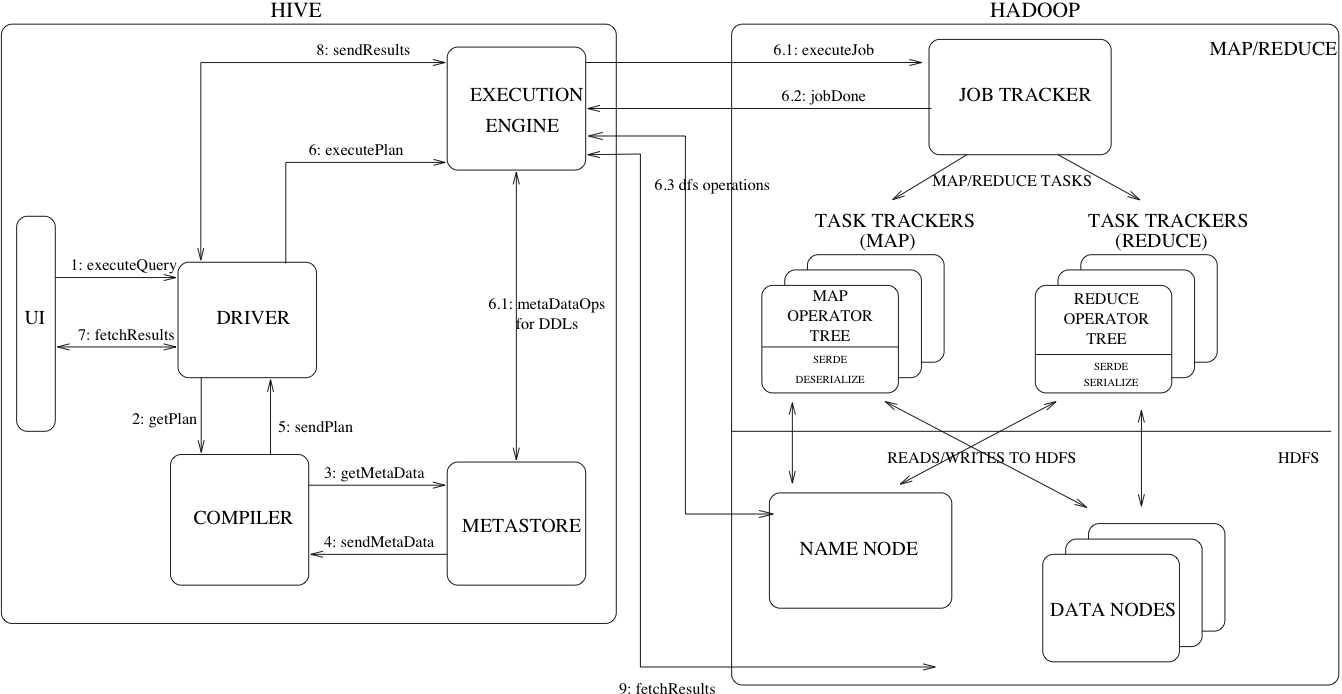
\includegraphics[width=0.9\textwidth]{system_architecture.png}
        \caption{HIVE Query Processing Workflow in Hadoop Ver.1 Environment}
        \label{fig01}
\end{figure*}

Other features of Hive include:
\bi
\ii Indexing to provide acceleration, index type including \textit{compaction} and \textit{Bitmap index} as of 0.10, more index types are planned.
\ii Different \textit{storage types} such as plain text, RCFile, HBase, ORC, and others.
\ii Metadata storage in an RDBMS, significantly reducing the time to perform \textit{semantic checks} during query execution.
\ii Operating on compressed data stored into the Hadoop ecosystem using algorithms including DEFLATE, BWT, snappy, etc.
\ii Built-in user defined functions (UDFs) to manipulate dates, strings, and other data-mining tools. Hive supports extending the UDF set to handle use-cases not supported by built-in functions.
\ii SQL-like queries (HiveQL), which are implicitly converted into MapReduce or Tez, or Spark jobs.
\ei

\section{Hive Architecture}
Figure \ref{fig01} shows the major components of Hive and its interactions with Hadoop. As shown in that figure, the main components of Hive are:
\bi
\ii \textit{User Interface} – The user interface for users to submit queries and other operations to the system. As of 2011 the system had a command line interface and a web based GUI was being developed.
\ii \textit{Driver} – The component which receives the queries. This component implements the notion of session handles and provides execute and fetch APIs modeled on JDBC/ODBC interfaces.
\ii \textit{Compiler} – The component that parses the query, does semantic analysis on the different query blocks and query expressions and eventually generates an execution plan with the help of the table and partition metadata looked up from the metastore.
\ii \textit{Metastore} – The component that stores all the structure information of the various tables and partitions in the warehouse including column and column type information, the serializers and deserializers necessary to read and write data and the corresponding HDFS files where the data is stored.
\ii \textit{Execution Engine} – The component which executes the execution plan created by the compiler. The plan is a DAG of stages. The execution engine manages the dependencies between these different stages of the plan and executes these stages on the appropriate system components.
\ei
Figure \ref{fig01} also shows how a typical query flows through the system. The UI calls the execute interface to the Driver (step 1 in Figure \ref{fig01}). 
The Driver creates a session handle for the query and sends the query to the compiler to generate an execution plan (step 2). 
The compiler gets the necessary metadata from the metastore (steps 3 and 4). 
This metadata is used to typecheck the expressions in the query tree as well as to prune partitions based on query predicates. 
The plan generated by the compiler (step 5) is a DAG of stages with each stage being either a map/reduce job, a metadata operation or an operation on HDFS. For map/reduce stages, the plan contains map operator trees (operator trees that are executed on the mappers) and a reduce operator tree (for operations that need reducers). 
The execution engine submits these stages to appropriate components (steps 6, 6.1, 6.2 and 6.3). 
In each task (mapper/reducer) the deserializer associated with the table or intermediate outputs is used to read the rows from HDFS files and these are passed through the associated operator tree. Once the output is generated, it is written to a temporary HDFS file though the serializer (this happens in the mapper in case the operation does not need a reduce). 
The temporary files are used to provide data to subsequent map/reduce stages of the plan. For DML operations the final temporary file is moved to the table's location. 
This scheme is used to ensure that dirty data is not read (file rename being an atomic operation in HDFS). For queries, the contents of the temporary file are read by the execution engine directly from HDFS as part of the fetch call from the Driver (steps 7, 8 and 9).

\section{Hive Data Model}
Data in Hive is organized into:
\bi
\ii \textit{Tables} – These are analogous to Tables in Relational Databases. Tables can be filtered, projected, joined and unioned. Additionally all the data of a table is stored in a directory in HDFS. Hive also supports the notion of external tables wherein a table can be created on prexisting files or directories in HDFS by providing the appropriate location to the table creation DDL. The rows in a table are organized into typed columns similar to Relational Databases.
\ii \textit{Partitions} – Each Table can have one or more partition keys which determine how the data is stored, for example a table T with a date partition column ds had files with data for a particular date stored in the $<$table location$>$/ds=$<$date$>$ directory in HDFS. Partitions allow the system to prune data to be inspected based on query predicates, for example a query that is interested in rows from T that satisfy the predicate T.ds = '2008-09-01' would only have to look at files in $<$table location$>$/ds=2008-09-01$/$ directory in HDFS.
\ii \textit{Buckets} – Data in each partition may in turn be divided into Buckets based on the hash of a column in the table. Each bucket is stored as a file in the partition directory. Bucketing allows the system to efficiently evaluate queries that depend on a sample of data (these are queries that use the SAMPLE clause on the table).
\ei

Apart from primitive column types (integers, floating point numbers, generic strings, dates and booleans), Hive also supports arrays and maps. Additionally, users can compose their own types programmatically from any of the primitives, collections or other user-defined types. 
The typing system is closely tied to the \textit{SerDe} (Serailization/Deserialization) and object inspector interfaces. User can create their own types by implementing their own object inspectors, and using these object inspectors they can create their own SerDes to serialize and deserialize their data into HDFS files). 
These two interfaces provide the necessary hooks to extend the capabilities of Hive when it comes to understanding other data formats and richer types. Builtin object inspectors like \textit{ListObjectInspector}, \textit{StructObjectInspector} and \textit{MapObjectInspector} provide the necessary primitives to compose richer types in an extensible manner. 
For maps (associative arrays) and arrays useful builtin functions like size and index operators are provided. The \textit{dotted} notation is used to navigate \textit{nested types}, for example a.b.c = 1 looks at field c of field b of type a and compares that with 1.

\section{Metastore}

\textbf{Motivation:} The \textit{Metastore} provides two important but often overlooked features of a data warehouse: 
\textit{data abstraction} and \textit{data discovery}. 
Without the data abstractions provided in Hive, a user has to provide information about data formats, extractors and loaders along with the query. In Hive, this information is given during table creation and reused every time the table is referenced. 
This is very similar to the traditional warehousing systems. The second functionality, data discovery, enables users to discover and explore relevant and specific data in the warehouse. Other tools can be built using this metadata to expose and possibly enhance the information about the data and its availability. 
Hive accomplishes both of these features by providing a \textit{metadata repository} that is tightly integrated with the Hive query processing system so that data and metadata are in sync.

\noindent
\textbf{Metadata Objects:}
The Metastore manages three types of metadata objects such as databases, tables, and partitions.
\bi 
\ii \textit{Database} – is a namespace for tables. It can be used as an administrative unit in the future. The database 'default' is used for tables with no user-supplied database name.
\ii \textit{Table} – Metadata for a table contains list of columns, owner, storage and SerDe information. It can also contain any user-supplied key and value data. Storage information includes location of the underlying data, file inout and output formats and bucketing information. SerDe metadata includes the implementation class of serializer and deserializer and any supporting information required by the implementation. All of this information can be provided during creation of the table.
\ii \textit{Partition} – Each partition can have its own columns and SerDe and storage information. This facilitates schema changes without affecting older partitions.
\ei

\noindent
\textbf{Metastore Architecture:} Metastore is an object store with a database or file backed store. The database backed store is implemented using an \textit{object-relational mapping} (ORM) solution called the DataNucleus. The prime motivation for storing this in a relational database is queriability of metadata. Some disadvantages of using a separate data store for metadata instead of using HDFS are synchronization and scalability issues. Additionally there is no clear way to implement an object store on top of HDFS due to lack of random updates to files. This, coupled with the advantages of queriability of a relational store, made our approach a sensible one.
The metastore can be configured to be used in a couple of ways: remote and embedded. In remote mode, the metastore is a Thrift service. This mode is useful for non-Java clients. In embedded mode, the Hive client directly connects to an underlying metastore using JDBC. This mode is useful because it avoids another system that needs to be maintained and monitored. Both of these modes can co-exist.

\noindent
\textbf{Metastore Interface:} Metastore provides a Thrift interface to manipulate and query Hive metadata. Thrift provides bindings in many popular languages. Third party tools can use this interface to integrate Hive metadata into other business metadata repositories.

\section{Hive Query Language}
HiveQL is an SQL-like query language for Hive. It mostly mimics SQL syntax for creation of tables, loading data into tables and querying the tables. HiveQL also allows users to embed their custom map-reduce scripts. These scripts can be written in any language using a simple row-based streaming interface – read rows from standard input and write out rows to standard output. This flexibility comes at a cost of a performance hit caused by converting rows from and to strings. However, we have seen that users do not mind this given that they can implement their scripts in the language of their choice. Another feature unique to HiveQL is multi-table insert. In this construct, users can perform multiple queries on the same input data using a single HiveQL query. Hive optimizes these queries to share the scan of the input data, thus increasing the throughput of these queries several orders of magnitude. We omit more details due to lack of space. For a more complete description of the HiveQL language see the language manual.

\subsection{Compiler}
Conceptual level architecture of the Hive can be decomposed into three major components; \textit{parser}, \textit{semantic analyzer}, and \textit{execution libraries}. And, execution libraries contain \textit{logical} plan generator, \textit{query} plan generator, \textit{optimizer}, and \textit{query executor}.

\bi
\ii \textit{Parser} – Transform a query string to a \textit{abstract syntax tree} (AST) representation. In order to parse a HiveQL, Hive exploits ANTLR (ANother Tool for Language Recognition) library as a parser generator, which is a powerful parser generator for reading, processing, executing, or translating structured text or binary files. The \textit{Hive.g} file defines keywords, tokens, translations from HiveQL to AST (see ASTNode.java). Every time \textit{Hive.g} is changed, you need to '\textit{ant clean}' first and rebuild using '\textit{ant package}'.
\ii \textit{Semantic Analyzer} – Transform the parse tree to an internal query representation, which is still \textit{block based} and not an operator tree. As part of this step, the column names are verified and expansions like * are performed. Type-checking and any implicit type conversions are also performed at this stage. If the table under consideration is a partitioned table, which is the common scenario, all the expressions for that table are collected so that they can be later used to prune the partitions which are not needed. If the query has specified sampling, that is also collected to be used later on. \textit{BaseSemanticAnalyzer} is the \textit{base class} for \textit{DDLSemanticAnalyzer} and \textit{SemanticAnalyzer}.
\textit{SemanticAnalyzer} handles queries, DML, and some DDL (create-table). \textit{DDLSemanticAnalyzer} handles alter table etc.
\ii \textit{Logical Plan Generator} – Convert the internal query representation to a logical plan, which consists of a tree of operators. 
\textit{SemanticAnalyzer.analyzeInternal()} is the main function for generating a logical plan.
The \textit{doPhase1()} methods recursively traverse AST tree and check for semantic errors and gather metadata which is put in \textit{QB} (Query Block) and \textit{QBParseInfo} as shown in Figure \ref{fig02} and \ref{fig03}. And, the \textit{getMetaData()} query metastore and get metadata for the data sources and put them into \textit{QB} and \textit{QBParseInfo}.
\begin{figure}[htb]
        \centering
        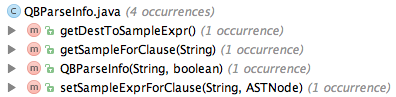
\includegraphics[width=0.48\textwidth]{qbparserinfo.png}
        \caption{QBParseInfo class}
        \label{fig02}
\end{figure}

The \textit{getPlan()}  takes the QB/QBParseInfo and AST tree and generate an operator tree. And, it is recursively called for each subqueries (QB), and output the root of the operator tree. For each subquery, \textit{getPlan()} create operators "\textit{bottom-up}" starting from FROM, WHERE, GROUPBY, ORDERBY, SELECT clauses. Actually, Hive code names each \textit{leaf} operator as "\textit{root}" and it \textit{downstream} operators as children.  In the FROM clause, generate a \textit{TableScanOperator} for each source table. 
\begin{figure}[htb]
        \centering
        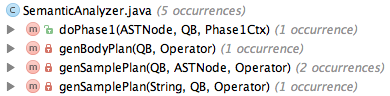
\includegraphics[width=0.48\textwidth]{semantic_analyzer.png}
        \caption{SemanticAnalyzer class}
        \label{fig03}
\end{figure}

The \textit{getBodyPlan()}  is then called to handle WHERE-GROUPBY-ORDERBY-SELECT clauses.
The \textit{genFilterPlan()} is a method  for WHERE clause. The  \textit{genGroupByPlanMapAgg1MR/2MR()} is a method for map-side partial aggregation.
The \textit{genGroupByPlan1MR/2MR()} is a method  for reduce-side aggregation. The  \textit{genSelectPlan()} is a method for SELECT-clause.
The \textit{genReduceSink()} is a method for marking the boundary between map/reduce phases. The \textit{genFileSink()} is a method  to store intermediate results. 

Some of the operators are \textit{relational algebra} operators like 'filter', 'join' etc. But some of the operators are Hive specific and are used later on to convert this plan into a series of map-reduce jobs. One such operator is a reduceSink operator which occurs at the map-reduce boundary. This step also includes the optimizer to transform the plan to improve performance – some of those transformations include: converting a series of joins into a single multi-way join, performing a map-side partial aggregation for a group-by, performing a group-by in 2 stages to avoid the scenario when a single reducer can become a bottleneck in presence of skewed data for the grouping key. Each operator comprises a descriptor which is a serializable object.
\ii \textit{Query Plan Generator} – Convert the logical plan to a series of map-reduce tasks. The operator tree is recursively traversed, to be broken up into a series of map-reduce serializable tasks which can be submitted later on to the map-reduce framework for the Hadoop distributed file system. The reduceSink operator is the map-reduce boundary, whose descriptor contains the reduction keys. The reduction keys in the reduceSink descriptor are used as the reduction keys in the map-reduce boundary. The plan consists of the required samples/partitions if the query specified so. The plan is serialized and written to a file. Finally, the resulting operator tree, along with other parsing info, is stored in \textit{ParseContext} and passed \textit{Optimizer} (see Optimizer.java).
\ei
 
\subsection{Optimizer}
Optimizer is a set of transformation rules on the operator tree. The transformation rules are specified by a \textit{regexp pattern} on the tree and a \textit{Worker/Dispatcher framework}.
More plan transformations are performed by the optimizer. The optimizer is an evolving component. As of 2011, it was \textit{rule-based} and performed the following: \textit{column pruning} and \textit{predicate pushdown}. 
Current Hive's rewrite rules include:
\textit{ColumnPruner, 
  PredicatePushDown,
  PartitionPruner,
  GroupByOptimizer, 
  SamplePruner,
  MapJoinProcessor,
  UnionProcessor,}
and \textit{JoinReorder} rules.
However, the infrastructure was in place, and there was work under progress to include other optimizations like map-side join and several \textit{join optimizations}.
 
The optimizer can be enhanced to be \textit{cost-based}. The sorted nature of output tables can also be preserved and used later on to generate better plans. The query can be performed on a small sample of data to guess the data distribution, which can be used to generate a better plan.
 A \textit{correlation optimizer} was added in Hive 0.12 \cite{Huai:2014}.
The plan is a generic operator tree, and can be easily manipulated.
The \textit{genMapRedWorks()} takes the \textit{QB/QBParseInfo} and the operator tree and generate a DAG of MapReduceTasks.
The generation is also based on the Worker/Dispatcher framework while traversing the operator tree.
The \textit{Validate() }on the physical plan is called at the end of \textit{Driver.compile()}.
 
\subsection{Execution}
\textit{Driver.execute} takes the output from \textit{Driver.compile} and prepare hadoop command line (in local mode) or call \textit{ExecDriver.execute} (in remote mode).
This execution contains the following procedures:
\bi
\ii Start a session.
\ii Execute \textit{PreExecutionHooks}.
\ii Create a \textit{Runnable} for each Task that can be executed in parallel and launch Threads within a certain limit.
\ii Monitor \textit{Thread status} and update \textit{Session}.
\ii Execute \textit{PostExecutionHooks}.
\ei
Hadoop jobs are started from \textit{MapRedTask.execute()} of \textit{MapRedTask} class as shown in Figure \ref{fig04}. 
The detail procedure for starting Hadoop MR jobs is as follows.
\bi
\ii Get info of all needed JAR files with \textit{ExecDriver} as the starting class.
\ii Serialize the Physical Plan (\textit{MapRedTask}) to an XML file.
\ii Gather other info such as Hadoop version and prepare the hadoop command line.
\ii Execute the hadoop command line in a separate process.
\ei 
\begin{figure}[htb]
        \centering
        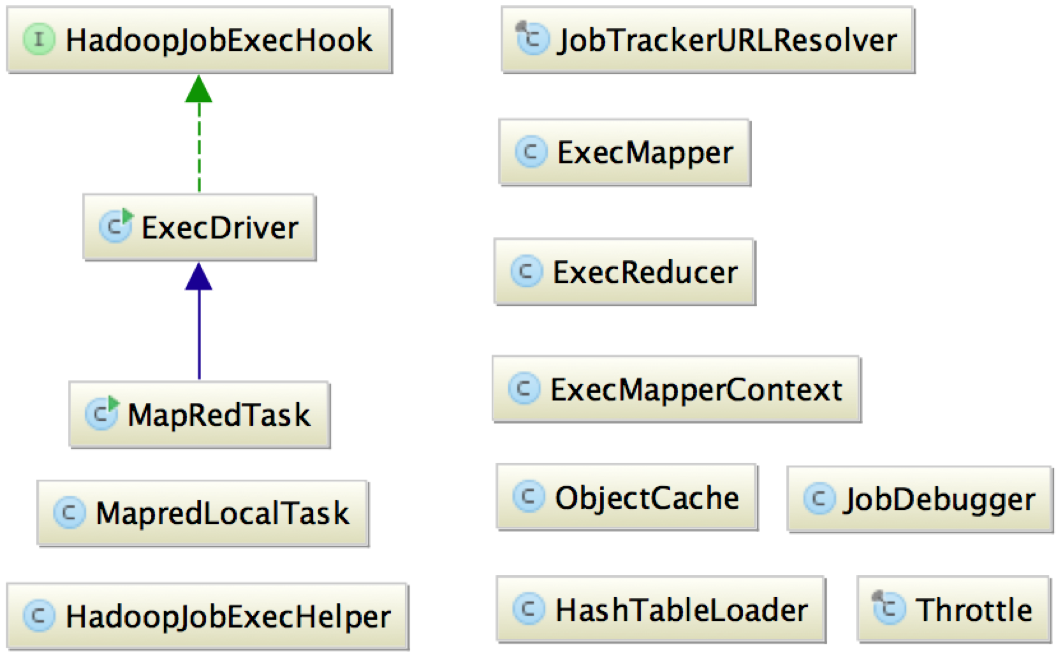
\includegraphics[width=0.48\textwidth]{mapredtask.png}
        \caption{Class diagram related to the MapRedTask class.}
        \label{fig04}
\end{figure}

In order to start Hadoop MR jobs, the \textit{ExecDriver} deserialize the plan from the XML file and call \textit{execute()}.
\textit{Execute()} set up the number of reducers, job scratch dir, the starting mapper class (\textit{ExecMapper}) and starting reducer class (\textit{ExecReducer}), and other info to JobConf and submit the job through \textit{hadoop.mapred.JobClient}.
The query plan is again serialized into a file and put into \textit{DistributedCache} to be sent out to mappers/reducers before the job is started.
\textit{ExecMapper} create a \textit{MapOperator} as the parent of all root operators in the query plan and start executing on the operator tree.
Each \textit{Operator} class comes with a descriptor class, which contains metadata passing from compilation to execution.
Any metadata variable that needs to be passed should have a public setter \& getter in order for the XML serializer/deserializer to work.

\section{Conclusion}
In this technical report, we presented a survey of the implementation details for query processing in Hive. Conceptual level architecture for query processing can be decomposed into three major components; \textit{parser}, \textit{semantic analyzer}, and \textit{execution libraries}. And, execution libraries contain \textit{logical} plan generator, \textit{query} plan generator, \textit{optimizer}, and \textit{query executor}.


The database community has been always focusing on dealing with the challenges of "Big Data" management, although the meaning "Big" has been evolving continuously to represent different scales over the time. 
In the era of "Big Data", future systems for parallel processing should also support efficient exploratory query processing and analysis. It is vital to provide efficient support for processing on subsets of the available data only. At the same time, it is important to provide fast retrieval of results that are \textit{indicative}, \textit{approximate} and guide the user to formulating the correct query.
Defining of \textit{domain-specific} big data systems is another important research direction that will need to be deeply investigated.

\bibliographystyle{abbrv}
\bibliography{sqlonhadoop}

\end{document}
